\subsubsection{x86: 4 argumenty}

\myparagraph{MSVC}

Gdy skompilujemy kod za pomocą MSVC 2010 Express, otrzymamy:

\begin{lstlisting}[style=customasmx86]
$SG3830	DB	'a=%d; b=%d; c=%d', 00H

...

	push	3
	push	2
	push	1
	push	OFFSET $SG3830
	call	_printf
	add	esp, 16					; 00000010H
\end{lstlisting}

Kod jest niemal identyczny z tym, który widzieliśmy w \emph{\HelloWorldSectionName}~(\myref{sec:helloworld}), lecz teraz argumenty funkcji \printf zostały odłożone na stos w odwrotnej kolejności. Pierwszy argument jest zapisywany jako ostatni.

Przy okazji, zmienna typu \Tint w środowisku 32-bitowym ma długość 32 bitów, czyli 4 bajtów.

Mamy więc 4 argumenty. $4*4 = 16$~---zajmują dokładnie 16 bajtów na stosie: 32-bitowy wskaźnik na łańcuch znaków i trzy liczby typu \Tint.

\myindex{x86!\Instructions!ADD}
\myindex{x86!\Registers!ESP}
\myindex{cdecl}
Gdy \glslink{stack pointer}{wskaźnik stosu} (rejestr \ESP) jest przywracany za pomocą \INS{ADD ESP, X} za wywołaniem funkcji, to często można określić liczbę argumentów, dzieląc X przez 4.

Oczywiście dotyczy to tylko konwencji wywołań \emph{cdecl} i środowiska 32-bitowego!

O konwencjach wywołań przeczytasz tutaj ~(\myref{sec:callingconventions}).

Kompilator, gdy kilka funkcji jest wywoływanych jedna za drugą, może połączyć kilka instrukcji \q{ADD ESP, X} w jedną i umieścić ją po ostatnim wywołaniu:

\begin{lstlisting}[style=customasmx86]
push a1
push a2
call ...
...
push a1
call ...
...
push a1
push a2
push a3
call ...
add esp, 24
\end{lstlisting}

Przykład prawdziwego kodu:

\lstinputlisting[caption=x86,style=customasmx86]{patterns/03_printf/x86/add_example_PL.lst}

\clearpage
\myparagraph{MSVC and \olly}
\myindex{\olly}

Skorzystajmy z \olly.
Jest to jeden z najpopularniejszych debuggerów pod win32, działających w trybie użytkownika.
Przykład skompilujemy w MSVC 2012 z opcją \GTT{/MD}, która oznacza dynamiczne linkowanie do \GTT{MSVCR*.DLL},
by łatwo można było rozpoznać zaimportowane funkcje w debuggerze.

Możemy załadować plik wykonywalny do \olly.
Pierwszy breakpoint jest w \GTT{ntdll.dll}, naciskamy
F9 (run).
Drugi breakpoint jest w kodzie \ac{CRT}.
Musimy odnaleźć funkcję \main.

Można to zrobić scrollując na samą górę kodu (MSVC umieszcza funkcję \main na samym początku sekcji kodu):
\begin{figure}[H]
\centering
\myincludegraphics{patterns/03_printf/x86/olly3_1.png}
\caption{\olly: sam początek funkcji \main}
\label{fig:printf3_olly_1}
\end{figure}

Klikamy na instrukcję \INS{PUSH EBP}, wciskamy F2 (ustaw breakpoint) i wciskamy F9 (run).
Dzięki temu przeskoczymy kod z \ac{CRT}, którym nie jesteśmy na razie zainteresowani.

\clearpage
Naciśnij F8 (\stepover) 6 razy, by przeskoczyć 6 kolejnych instrukcji:

\begin{figure}[H]
\centering
\myincludegraphics{patterns/03_printf/x86/olly3_2.png}
\caption{\olly: przed wykonaniem \printf}
\label{fig:printf3_olly_2}
\end{figure}

\ac{PC} pokazuje teraz na instrukcję \INS{CALL printf}.
\olly, jak inne debuggery, podświetla rejestry, które zostały zmienione.
Za każdym razem, gdy naciskasz F8, \EIP zmienia się i jego wartość jest wyświetlana na czerwono. \ESP również się zmienia, gdyż argumenty są przekazywane przez stos.\\
\\
Gdzie na stosie są nasze wartości?
Spójrz na obszar w prawym, dolnym rogu okna:

\begin{figure}[H]
\centering
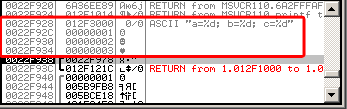
\includegraphics[width=0.5\textwidth]{patterns/03_printf/x86/olly3_stack.png}

\caption{\olly: stos po odłożeniu argumentów (czerwona ramka została dodana przez autora w programie graficznym)}
\end{figure}

Widzimy 3 kolumny: adres na stosie, wartość i dodatkowo komentarz \olly.
\olly rozumie wskaźniki na łańcuchy znaków, więc wypisuje wartość tego łańcucha jako komentarz .

Możesz kliknąć prawym przyciskiem myszy na łańcuch znaków z formatem i wybrać \q{Follow in dump}.
Łańcuch znaków pojawi się w lewym, dolnym oknie debuggera, wyświetlającym zawartość pamięci.
Możesz ją tam edytować.
Mógłbyś zmienić format łańcucha znaków, tak by na wyjście został wypisany inny tekst.
W tym przykładzie nie jest to użyteczna funkcjonalność, ale możesz jej użyć w ramach ćwiczeń, by lepiej poznać opisane wcześniej mechanizmy.

\clearpage
Wciśnij F8 (\stepover).

Zobaczymy następujący rezultat w konsoli:

\lstinputlisting{patterns/03_printf/x86/console.txt}

Sprawdźmy jak zmieniły się rejestry i stos:

\begin{figure}[H]
\centering
\myincludegraphics{patterns/03_printf/x86/olly3_3.png}
\caption{\olly po wykonaniu funkcji \printf{}}
\label{fig:printf3_olly_3}
\end{figure}

Rejestr \EAX zawiera teraz \GTT{0xD} (13).
Jest to spodziewana wartość, ponieważ \printf zwraca liczbę wypisanych znaków.
Zmieniła się wartość \EIP: zawiera teraz adres kolejnej instrukcji, występującej bezpośrednio za \INS{CALL printf}.
\ECX i \EDX również się zmieniły.
Najwyraźniej implementacja \printf wykorzystała je do własnych celów.

Ważnym faktem jest to, że ani wartość \ESP, ani stan stosu się nie zmieniły!

Łatwo zauważyć, że łańcuch znaków z formatem oraz 3 powiązane z nim argumentu wciąż tam są. Jest to konwencja wywoływania \emph{cdecl}: \glslink{callee}{funkcja wywoływana} nie przywraca \ESP do pierwotnego stanu.
Ta odpowiedzialność spoczywa na \glslink{caller}{wywołującym}.

\clearpage
Ponownie wciśnij F8, by wykonać instrukcję \INS{ADD ESP, 10}:

\begin{figure}[H]
\centering
\myincludegraphics{patterns/03_printf/x86/olly3_4.png}
\caption{\olly: po wykonaniu instrukcji \INS{ADD ESP, 10}}
\label{fig:printf3_olly_4}
\end{figure}

Zmieniła się wartość \ESP, ale wartości na stosie zostały niezmienione!
Można się tego spodziewać; nikt nie musi ich nadpisywać.
Wszystko powyżej wskaźnika stosu (\ac{SP}) to \emph{szum} czy \emph{\garbage{}} i nie ma znaczenia.
Czyszczenie nieużywanych wpisów na stosie byłoby stratą czasu i nikt tego nie potrzebuje.
% chyba, że są tam wrażliwe dane, które nie powinny być odtwarzane?

\myparagraph{GCC}

Skompilujmy ten sam program na Linuksie, za pomocą GCC 4.4.1 i sprawdźmy wynik w programie \IDA:

\lstinputlisting[style=customasmx86]{patterns/03_printf/x86/x86_1.asm}

Jedyną zauważalną różnicą jest inny sposób odkładania argumentów na stos.
W tym przykładzie GCC explicite podaje adres w obrębie stosu i nie używa instrukcji \PUSH/\POP.

\myparagraph{GCC i GDB}
\myindex{GDB}

Wczytajmy plik wykonywalny do debuggera \ac{GDB}.

Opcja \GTT{-g} sprawia, że kompilator zapisuje do pliku wykonywalnego informacje użyteczne do debuggowania.

\begin{lstlisting}
$ gcc 1.c -g -o 1
\end{lstlisting}

\begin{lstlisting}
$ gdb 1
GNU gdb (GDB) 7.6.1-ubuntu
...
Reading symbols from /home/dennis/polygon/1...done.
\end{lstlisting}

\begin{lstlisting}[caption=Ustawmy breakpoint w funkcji \printf]
(gdb) b printf
Breakpoint 1 at 0x80482f0
\end{lstlisting}

Kontynuujmy wykonywanie kodu.
Gdybyśmy dysponowali kodem źródłowym funkcji \printf, \ac{GDB} mógłby go wyświetlić obok instrukcji asemblera.

\begin{lstlisting}
(gdb) run
Starting program: /home/dennis/polygon/1

Breakpoint 1, __printf (format=0x80484f0 "a=%d; b=%d; c=%d") at printf.c:29
29	printf.c: No such file or directory.
\end{lstlisting}

Wypiszmy 10 wartości ze stosu. Skrajna lewa kolumna oznacza adres, pod którym wartości ze stosu znajdują się w pamięci.

\begin{lstlisting}
(gdb) x/10w $esp
0xbffff11c:	0x0804844a	0x080484f0	0x00000001	0x00000002
0xbffff12c:	0x00000003	0x08048460	0x00000000	0x00000000
0xbffff13c:	0xb7e29905	0x00000001
\end{lstlisting}

Pierwszy element to adres powrotu (\ac{RA}) (\GTT{0x0804844a}).
Możemy to sprawdzić, deasemblując pamięć pod tym adresem (instruujemy GDB, by wypisał 5 elementów ze stosu, interpretując je jako instrukcje asemblera):

\begin{lstlisting}[label=NOP_as_XCHG_example,style=customasmx86]
(gdb) x/5i 0x0804844a
   0x804844a <main+45>:	mov    $0x0,%eax
   0x804844f <main+50>:	leave
   0x8048450 <main+51>:	ret
   0x8048451:	xchg   %ax,%ax
   0x8048453:	xchg   %ax,%ax
\end{lstlisting}

Pojawiająca się dwa razy \INS{XCHG} działa jak pusta instrukcja \ac{NOP}, gdyż w tym przypadku ustawia wartość rejestr AX na jego bieżącą wartość.

Drugim elementem jest (\GTT{0x080484f0}) ~--- to adres łańcucha znaków z formatem:

\begin{lstlisting}
(gdb) x/s 0x080484f0
0x80484f0:	"a=%d; b=%d; c=%d"
\end{lstlisting}

Kolejne 3 elementy (1, 2, 3) to argumenty funkcji \printf.
Pozostałe elementy to prawdopodobnie \q{śmieci} znajdujące się na stosie,
lecz mogłyby to być wartości używane przez inne funkcje, ich zmienne lokalnce, etc.
Możemy je na razie zignorować.

Kontynuujmy za pomocą \q{finish}.
Polecenie powoduje, że GDB wykona wszystkie instrukcje aż do końca funkcji.
W tym przypadku do końca funkcji \printf.

\begin{lstlisting}
(gdb) finish
Run till exit from #0  __printf (format=0x80484f0 "a=%d; b=%d; c=%d") at printf.c:29
main () at 1.c:6
6		return 0;
Value returned is $2 = 13
\end{lstlisting}

\ac{GDB} pokazuje jaką wartość \printf zwróciła przez rejestr \EAX (13).
Jest to liczba znaków, które zostały wypisane i jest to dokładnie tyle, ile widzieliśmy w przykładzie z \olly.

Widzimy również \q{return 0;} wraz z informacją, że to wyrażenie jest w pliku \GTT{1.c}, w linii 6.
Plik \GTT{1.c} znajduje się w bieżącym katalogu i tam \ac{GDB} znalazł ten łańcuch znaków.
Skąd debugger wiedział, która linia kodu w C jest właśnie wykonywana?
Kompilatory, gdy generują informacje dla debuggera, zapisują również tablicę z zależnościami między liniami kodu źródłowego a adresami instrukcji,
GDB jest w końcu debuggerem pracującym z kodem źródłowym.

Przyjrzyjmy się rejestrom. W \EAX znajduje się wartość 13:

\begin{lstlisting}
(gdb) info registers
eax            0xd	13
ecx            0x0	0
edx            0x0	0
ebx            0xb7fc0000	-1208221696
esp            0xbffff120	0xbffff120
ebp            0xbffff138	0xbffff138
esi            0x0	0
edi            0x0	0
eip            0x804844a	0x804844a <main+45>
...
\end{lstlisting}

Deasemblujemy kolejne instrukcje.
Strzałka pokazuje na instrukcję, która zostanie wykonana jako kolejna.

\begin{lstlisting}[style=customasmx86]
(gdb) disas
Dump of assembler code for function main:
   0x0804841d <+0>:	push   %ebp
   0x0804841e <+1>:	mov    %esp,%ebp
   0x08048420 <+3>:	and    $0xfffffff0,%esp
   0x08048423 <+6>:	sub    $0x10,%esp
   0x08048426 <+9>:	movl   $0x3,0xc(%esp)
   0x0804842e <+17>:	movl   $0x2,0x8(%esp)
   0x08048436 <+25>:	movl   $0x1,0x4(%esp)
   0x0804843e <+33>:	movl   $0x80484f0,(%esp)
   0x08048445 <+40>:	call   0x80482f0 <printf@plt>
=> 0x0804844a <+45>:	mov    $0x0,%eax
   0x0804844f <+50>:	leave
   0x08048450 <+51>:	ret
End of assembler dump.
\end{lstlisting}

\ac{GDB} używa domyślnie składni AT\&T.
Możemy jednak przełączyć się na składnię Intela.

\begin{lstlisting}[style=customasmx86]
(gdb) set disassembly-flavor intel
(gdb) disas
Dump of assembler code for function main:
   0x0804841d <+0>:	push   ebp
   0x0804841e <+1>:	mov    ebp,esp
   0x08048420 <+3>:	and    esp,0xfffffff0
   0x08048423 <+6>:	sub    esp,0x10
   0x08048426 <+9>:	mov    DWORD PTR [esp+0xc],0x3
   0x0804842e <+17>:	mov    DWORD PTR [esp+0x8],0x2
   0x08048436 <+25>:	mov    DWORD PTR [esp+0x4],0x1
   0x0804843e <+33>:	mov    DWORD PTR [esp],0x80484f0
   0x08048445 <+40>:	call   0x80482f0 <printf@plt>
=> 0x0804844a <+45>:	mov    eax,0x0
   0x0804844f <+50>:	leave
   0x08048450 <+51>:	ret
End of assembler dump.
\end{lstlisting}

Wykonajmy kolejną linię kodu w \CCpp{}.
\ac{GDB} pokazuje klamrowy nawias zamykający, który oznacza koniec bloku kodu.

\begin{lstlisting}
(gdb) step
7	};
\end{lstlisting}

Sprawdźmy rejestry po wykonaniu instrukcji \INS{MOV EAX, 0}. Tak jak się spodziewamy, \EAX zawiera teraz wartość 0.

\begin{lstlisting}
(gdb) info registers
eax            0x0	0
ecx            0x0	0
edx            0x0	0
ebx            0xb7fc0000	-1208221696
esp            0xbffff120	0xbffff120
ebp            0xbffff138	0xbffff138
esi            0x0	0
edi            0x0	0
eip            0x804844f	0x804844f <main+50>
...
\end{lstlisting}
